\section{Stellar and halo mass estimates}\label{sec:stellar-mass}

The stellar masses of the lens galaxies are derived by comparison of
the photometric data with M/L estimates from population synthesis
models.  In principle, a detailed analysis of the spectral energy
distribution is needed to derive accurate stellar masses
\citep[e.g.][]{2009ApJS..185..253G,2011MNRAS.418.1587T}.
However, estimates to within 0.3\,dex in $\log($M$_s$/M$_\odot)$ can be
derived with a single colour, preferably tracing a rest-frame colour
similar to $U-V$ \citep[see fig.~1 of][]{2008MNRAS.383..857F}. This
paper presents a pilot study of the potential of SpaghettiLens to
constrain the physical properties of strong lenses. Therefore, we
further simplify the analysis by assuming a relationship between the
apparent total magnitude and stellar mass, at the redshift of the
lens. Note that for typical stellar population parameters, the
variation of this relation is at most 1\,dex. In this work, we make
use of the \citet{2003MNRAS.344.1000B} models to derive two functional
forms of the stellar mass with respect to SDSS-$i$ band
magnitudes. The models have solar metallicity, with a Chabrier
IMF, and assume two different age trends: a ``young'' model, with a
constant 500\,Myr age at all redshifts, and an ``old'' model where the
age is the oldest one possible at each redshift, adopting a
standard $\Lambda$CDM model with $H_0=70$\,km\,s$^{-1}$\,Mpc$^{-1}$
and $\Omega_m=0.3$. We take a geometric mean of the output from these
two models as the stellar mass of the lens. This rough estimate will
be improved in future versions by use of the available optical and NIR
magnitudes to derive more accurate constrains on the stellar
populations.

In addition, we also derive halo masses for the lenses by use of the
standard abundance matching technique, whereby a comparison of the
observed stellar mass function of galaxies with the dark matter halo
mass function from N-body simulations results in a simple relation
between the two. We emphasize that this derivation of halo mass should
be considered an ``average'' estimate, and a significant scatter can
be expected as galaxies with the same stellar mass can be found in
different environments. We refer the reader to \cite{2012MNRAS.424..104L}
for an assessment of the effect of abundance matching on the
derivation of dark matter halo properties in lensing galaxies. We
follow the prescription of \citet{2010ApJ...710..903M}, namely:

\begin{equation}
\begin{aligned}
\frac{\Mstel}{\Mhalo} &= \frac{2C_0}{(\Mhalo/M_1)^{-\beta} +
                                     (\Mhalo/M_1)^\gamma} \\
C_0 &= 0.02820, \quad M_1 = 10^{11.884} M_\odot \\
\beta &= 1.057, \quad \gamma = 0.556.
\end{aligned}
\end{equation}
and define a halo-matching index:
\begin{equation}
\haloindex = \frac{\ln(M/\Mstel)}{\ln(\Mhalo/\Mstel)}
\end{equation}
that relates the observed lensing to stellar mass, with the
global ratio expected if the host halo corresponds to the
average value derived by abundance matching. Several cases
for $\haloindex$ can be considered:
\begin{itemize}
\item $\haloindex < 0$ is unphysical because $M<\Mstel$.
\item $\haloindex = 0$ is when the stellar mass exactly accounts for the
  lensing mass.
\item $0 < \haloindex < 1$ is the typical situation, where the lens
  includes stars and dark matter, but not the full halo.
\item $\haloindex = 1$ means that the lens consists of the entire halo.
\item $\haloindex > 1$ is in tension with abundance-matching, because the
  lensing mass exceeds the expected halo mass.
\end{itemize}

\begin{figure*}
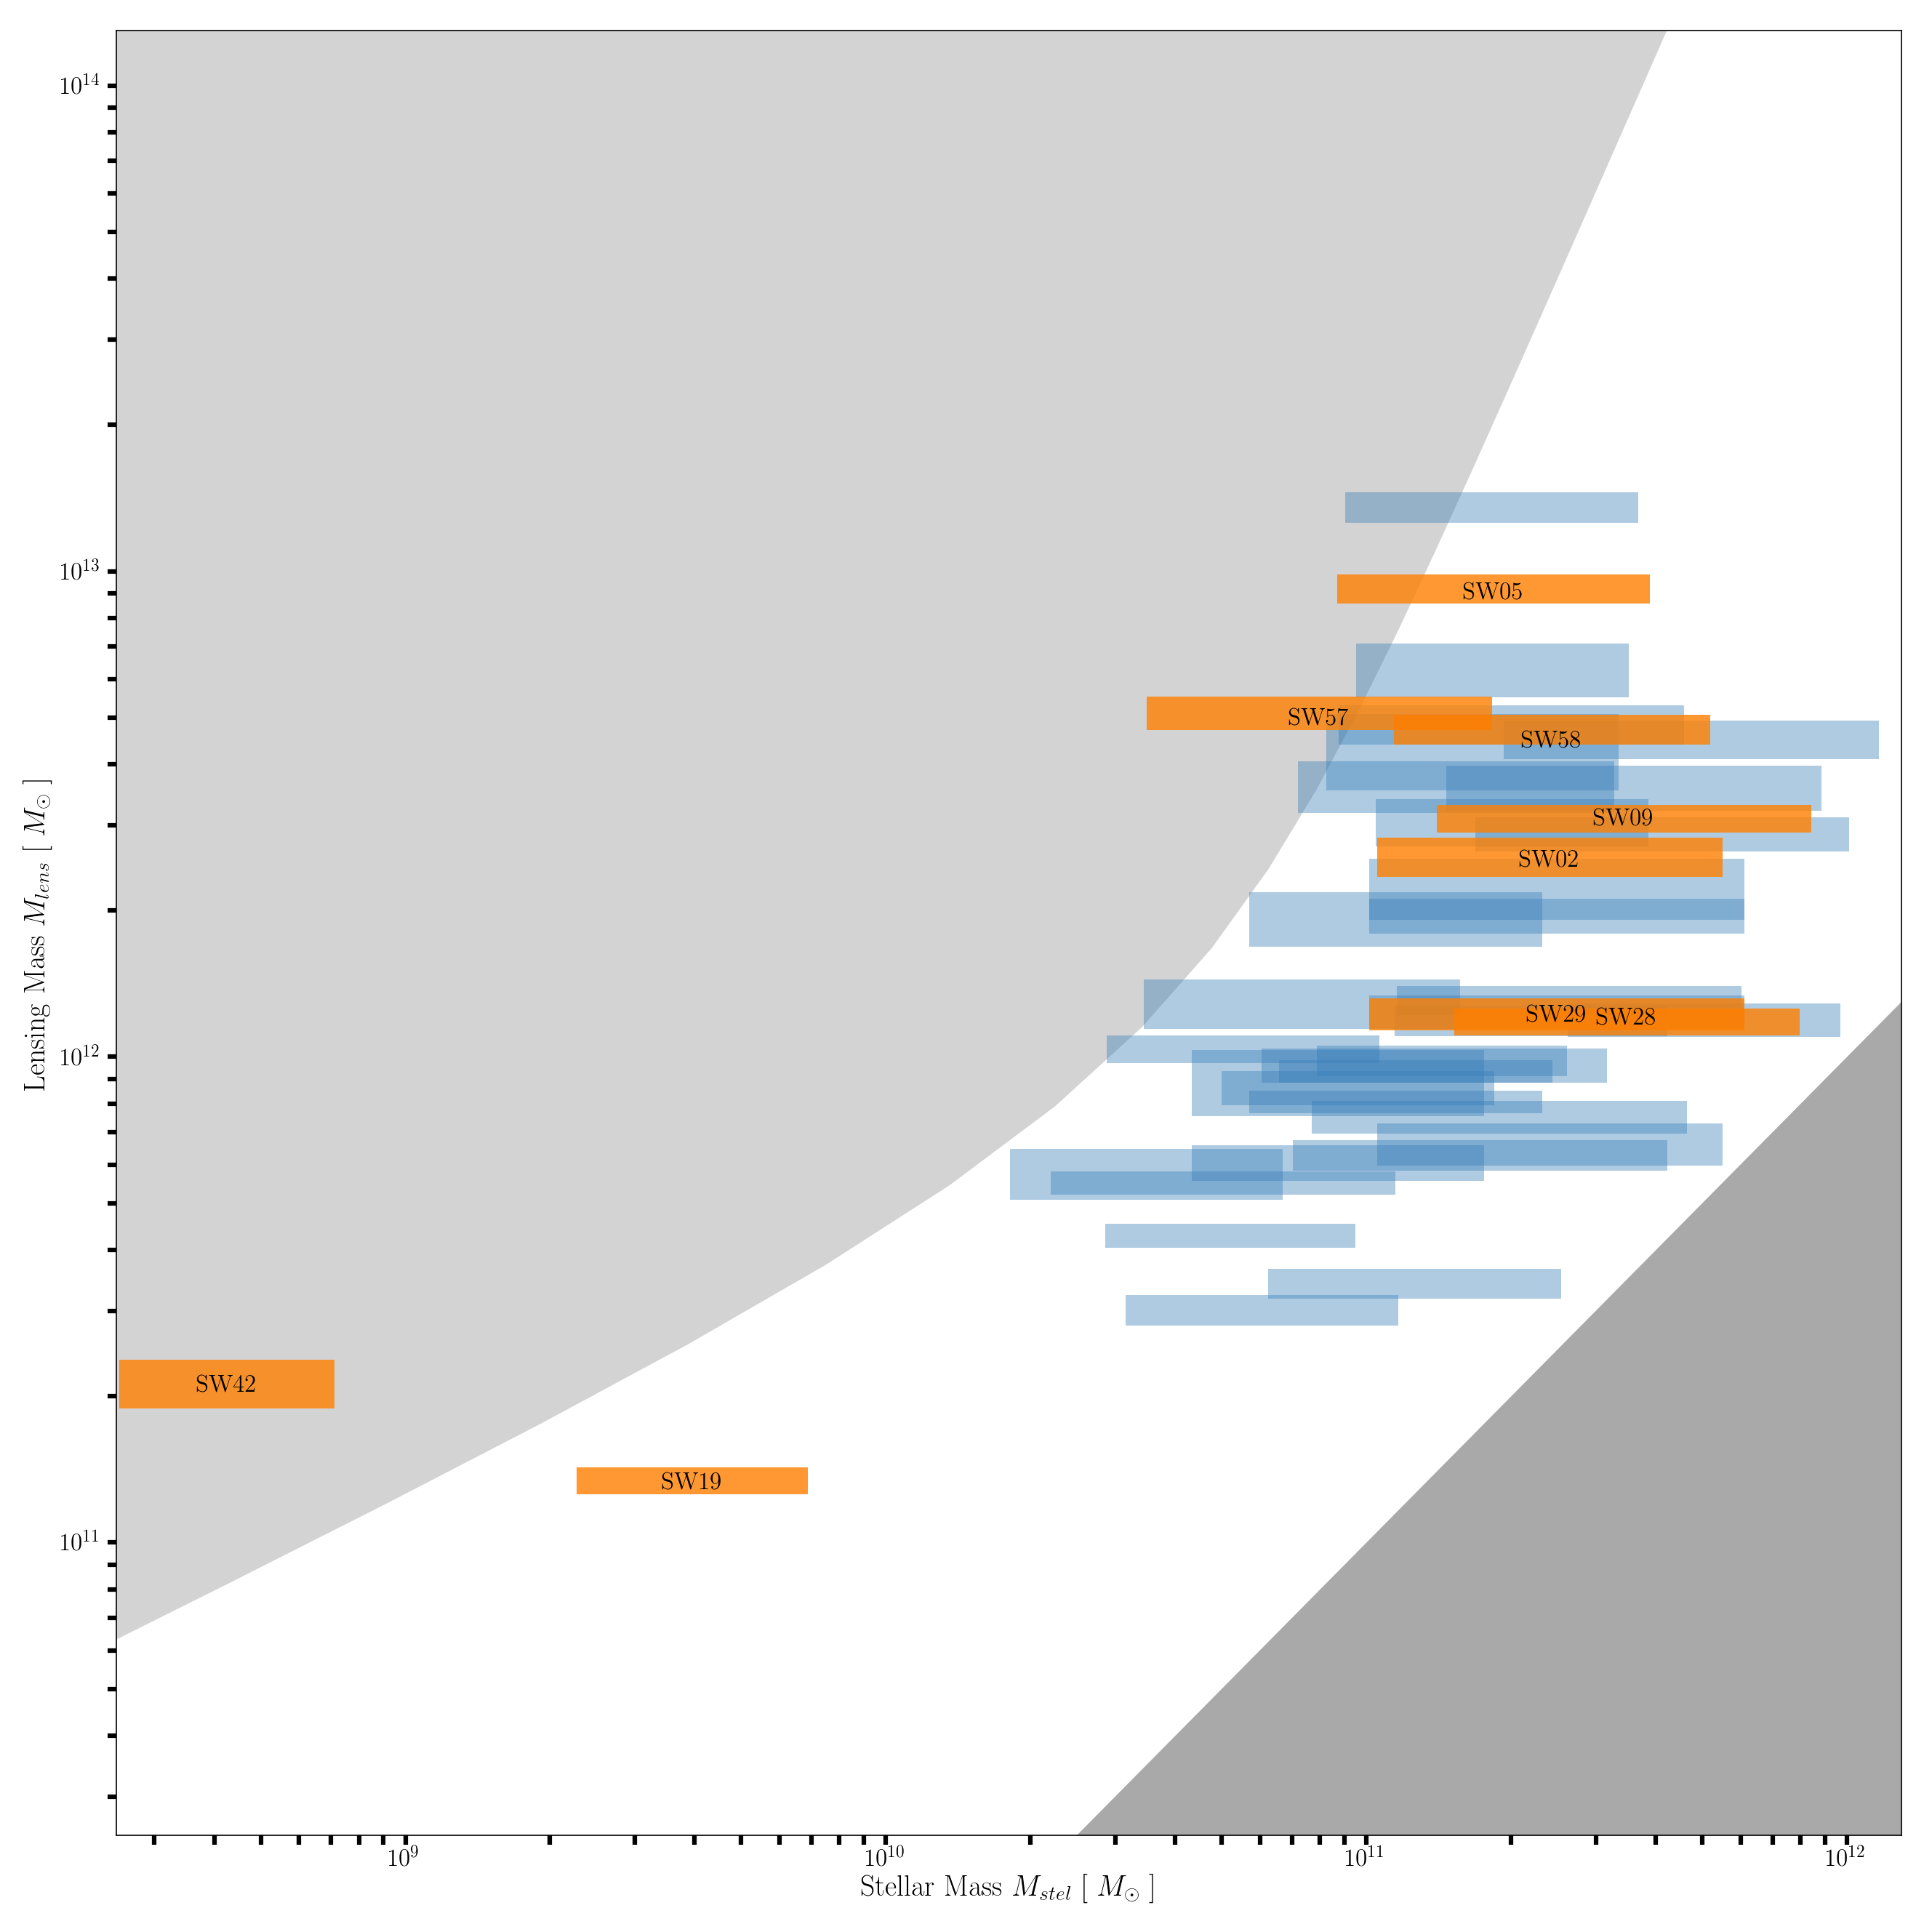
\includegraphics[width=\linewidth]{img/mlens_vs_mstel_one/mstel_vs_mtot_one}
\caption{}
\end{figure*}

